\section*{Exercise 1}

\subsection*{Part A}

PEAS descriptions for a robot basketball player, industrial orange-apple sorter and a stock investor are given in Table \ref{table:peas}.

\begin{table}[htpb]
\centering
\makebox{
\resizebox{!}{4cm}{\begin{tabular}{l p{5cm} p{5cm} p{5cm}}
\hline
\textbf{Agent Type} & Robot Basketball Player & Industrial Orange-Apple Sorter & Stock Investor \\
\hline
\up \textbox{\textbf{Performance} \\ \textbf{Measure}} & 

\begin{itemize}[leftmargin=*,noitemsep,topsep=0pt]
\item win \%
\item goals made / goals attempted \%
\item average points per game
\item performance index rating
\end{itemize} & 

\begin{itemize}[leftmargin=*,topsep=0pt,noitemsep]
\item accuracy \%
\item # fruits per second
\end{itemize} & 

\begin{itemize}[leftmargin=*,topsep=0pt,noitemsep]
\item average ROI
\item total earnings (or losses)
\item earnings per month/year
\end{itemize} \\
\hline
\up \textbf{Environment} &

\begin{itemize}[leftmargin=*,topsep=0pt,noitemsep]
\item basketball court
\item other agents (teammates and opponents)
\end{itemize} & 

\begin{itemize}[leftmargin=*,topsep=0pt,noitemsep]
\item conveyor belt and surrounding parts of engine
\item reception of sorted fruits (holes, boxes)
\end{itemize} & 

\begin{itemize}[leftmargin=*,topsep=0pt,noitemsep]
\item online stock markets
\item other agents (investors)
\end{itemize} \\
\hline
\up \textbf{Actuators} & & & \\
\hline
\up \textbf{Sensors} & & & \\
\hline
\end{tabular}}
}
\caption{������� ����� ������� ���������� ��� ����� ��� $�$ ����������� ���� �������.}
\label{table:peas}
\end{table}


\subsection*{Part B}

Table \ref{table:environments} contains the environmental characteristics of the three aforementioned agent types. In the following paragraphs I select a suitable agent design, providing a brief explanation for each agent type.


\begin{table}[htpb]
\centering
\makebox{
\resizebox{!}{3.4cm}{\begin{tabular}{l p{5cm} p{5cm} p{5cm}}
\hline
\textbf{Characteristic} & Robot Basketball Player & Industrial Orange - Apple Sorter & Stock Investor \\
\hline
\up \textbox{\textbf{Observable}} & partial (court not entirely observable) & partial (e.g. fruit not entirely observable internally) & partial (too many markets, stocks and investors)   \\
\hline
\up \textbf{Determinism} & stochastic (e.g. shot/pass curve) & stochastic (e.g. photo background) & deterministic* (it depends on how the affecting sociopolitical conditions are modeled)/ strategic (during negotiations against other agents) \\
\hline
\up \textbf{Dependency} & sequential & episodic (each fruit checked separately) & sequential \\
\hline
\up \textbf{Dynamicity} & dynamic & semidynamic (fruit type does not change but performance depends on time) & dynamic (stock prices and financial conditions can fluctuate too rapidly to be considered static) \\
\hline
\up \textbf{Description} & continuous & continuous & continuous \\
\hline
\up \textbf{Cardinality} & multiagent & single agent & multiagent\\
\hline
\end{tabular}}
}
\caption{Characteristics of the environment of three agent types.}
\label{table:environments}
\end{table}

\textbf{Robot basketball player:} \textit{Simple reflex agents} cannot perform well in this partially observable, dynamic environment. An \textit{internal-state model} could be used, but we would need many states that are difficult to define in such a continuous-state environment. In addition, simply storing the current state of the system would not be enough for the player to decide its next course of action. Furthermore, a \textit{goal-based agent} would be inefficient since scoring is not the only goal in basketball. Therefore, \textit{a utility-based model} is deemed necessary to provide a more efficient performance measure in this multiagent environment. Online \textit{learning} could also be applied during the match, allowing adaptation against the opposing team. Its application however would be difficult without sacrificing (at least their initial) performance.

\textbf{Industrial orange-apple sorter:} An \textit{internal-state model} would be enough for fruit classification based on the partially observable fruits and stochastic background (e.g. varying light in the room or existing branches/leaves). \textit{Learning} would be useful if we wanted our agent to classify more types of fruits in the future.

\textbf{Stock investor:} Similar to a robot basketball player, this agent needs to consider not only its basic goal of maximizing its net profit (namely buying cheaply and selling expensively), but also other features such as credibility, financial forecasts and cooperation with other investors. Therefore, a \textit{utility-based agent} would again be more appropriate. \textit{Learning} could also be proven useful in adaptation against opposing agents and new financial, cultural and political conditions.



\section*{Exercise 2}

\subsection*{Part A}

The solution is given in Figure \ref{fig:exercise2}.

\begin{figure}[htpb]
\centering
\makebox[\textwidth]{%
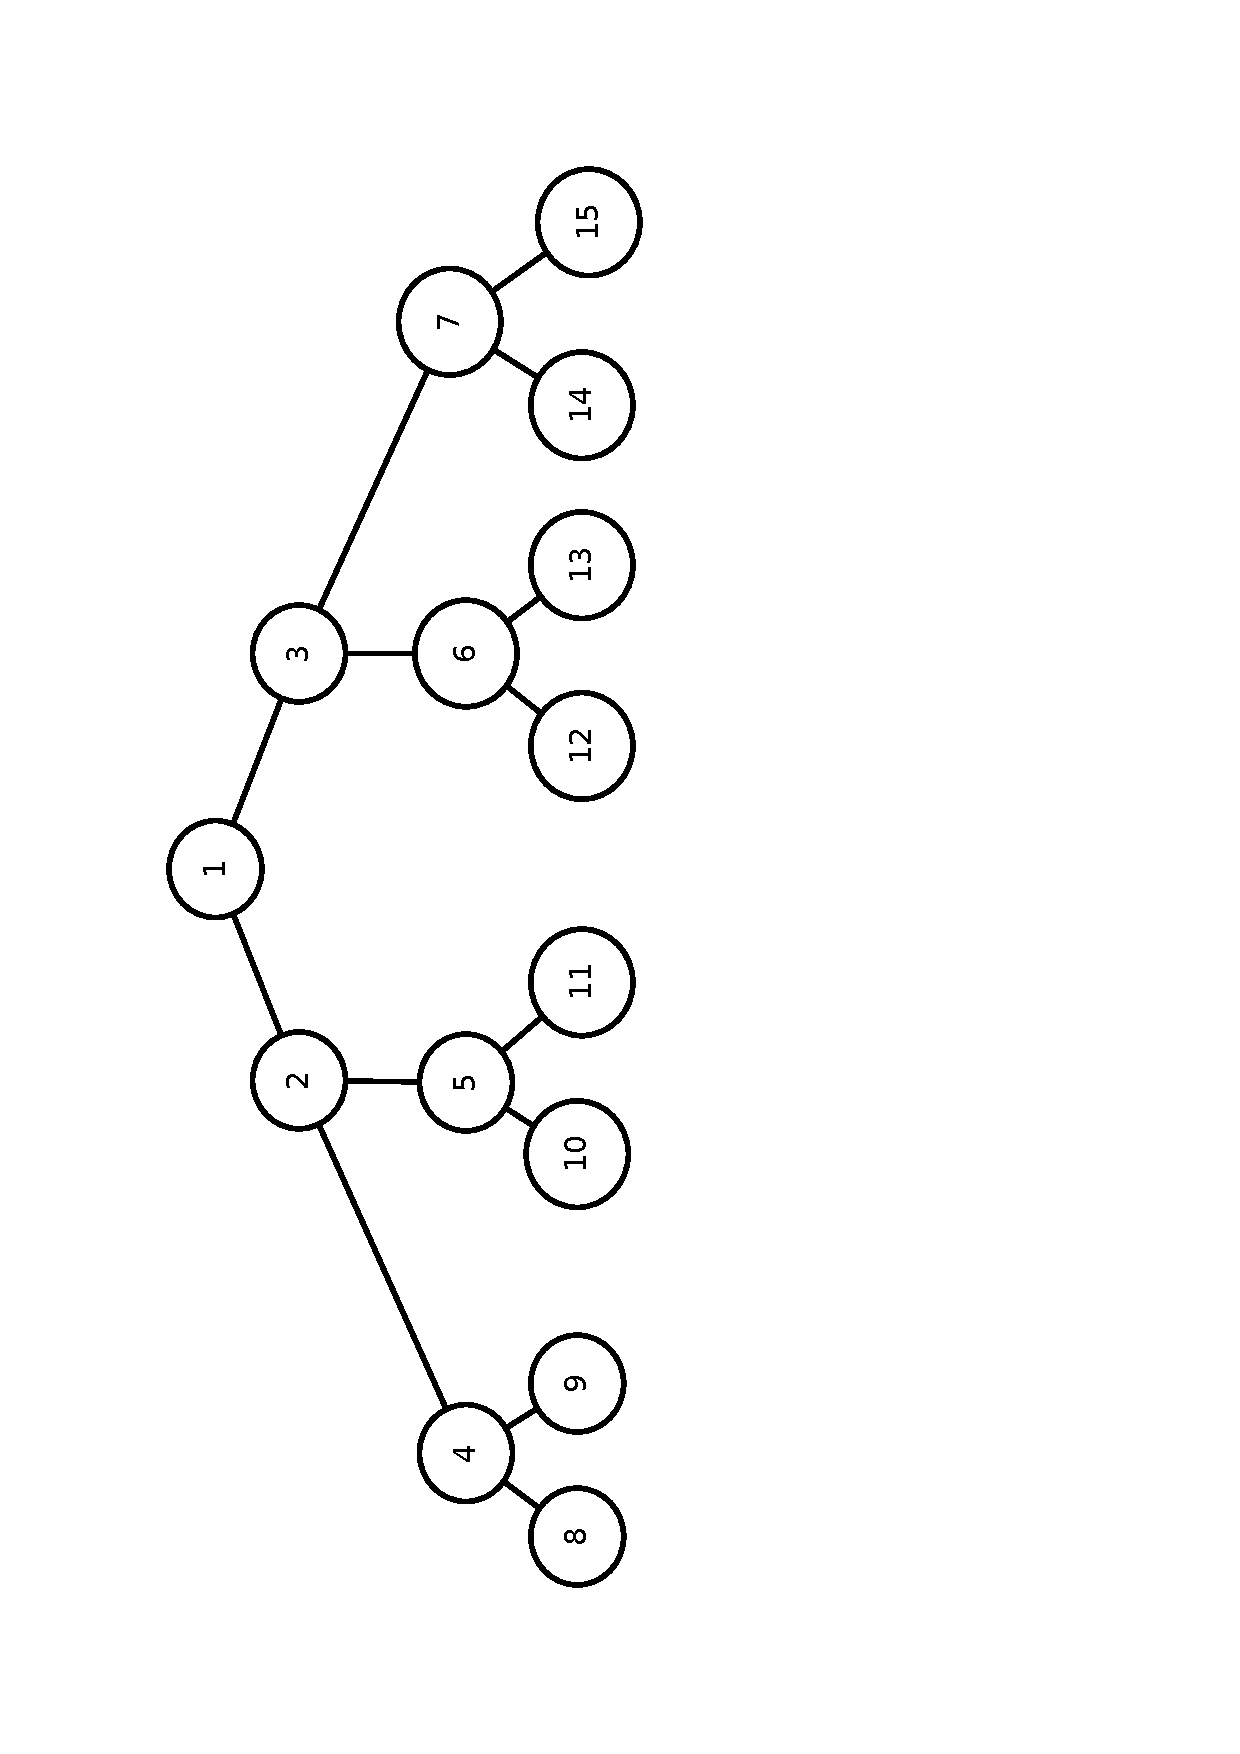
\includegraphics[width=0.3\textwidth, angle =-90, trim = 25mm 25mm 100mm 25mm,clip=true]{images/exercise2.pdf}}
\caption{State space for states 1 to 15, starting from 1, while the successor function returning two states, $2n$ and $2n+1$.}
\label{fig:exercise2}
% Place the label just after the caption to make the link work
\end{figure} % table makes a floating object with a title

\subsection*{Part B}

The order in which the nodes will be visited for each type of search is given below:

\begin{itemize}

\item Breadth-First Search: 1, 2, 3, 4, 5, 6, 7, 8, 9, 10, 11

\item Depth-Limited Search (depth limit 3): 1, 2, 4, 8, 9, 5, 10, 11

\item Iterative Deepening Search: (depth limit 0) 1 - (depth limit 1) 1, 2, 3 - (depth limit 2) 1, 2, 4, 5, 3, 6, 7 - (depth limit 3) 1, 2, 4, 8, 9, 5, 10, 11

\end{itemize}

\subsection*{Part C}

Bidirectional search would be quite appropriate for this problem, since we could easily employ the inverse of the successor function for searching in the opposite direction (from goal to start state): $\lfloor n/2 \rfloor$. For example, the bidirectional search algorithm would work as follows:

\begin{itemize}

\item Search from start: 1, 2, 3

\item Search from goal: 11, 5, (2)

\end{itemize}

The algorithm would terminate when the search from goal reaches node 2, which would have already been reached by the search from start. The final solution would therefore be 1, 2, 5, 11.

Simple search from goal to start would actually allow us to avoid searching altogether because each node has only a single predecessor. Hence, the solution could simply be found in $\log_2{n}$ steps.

\section*{Exercise 3}

The solution is given in Figure \ref{fig:exercise3}.

\begin{sidewaysfigure}[htpb]
\centering
\makebox[\textwidth]{%
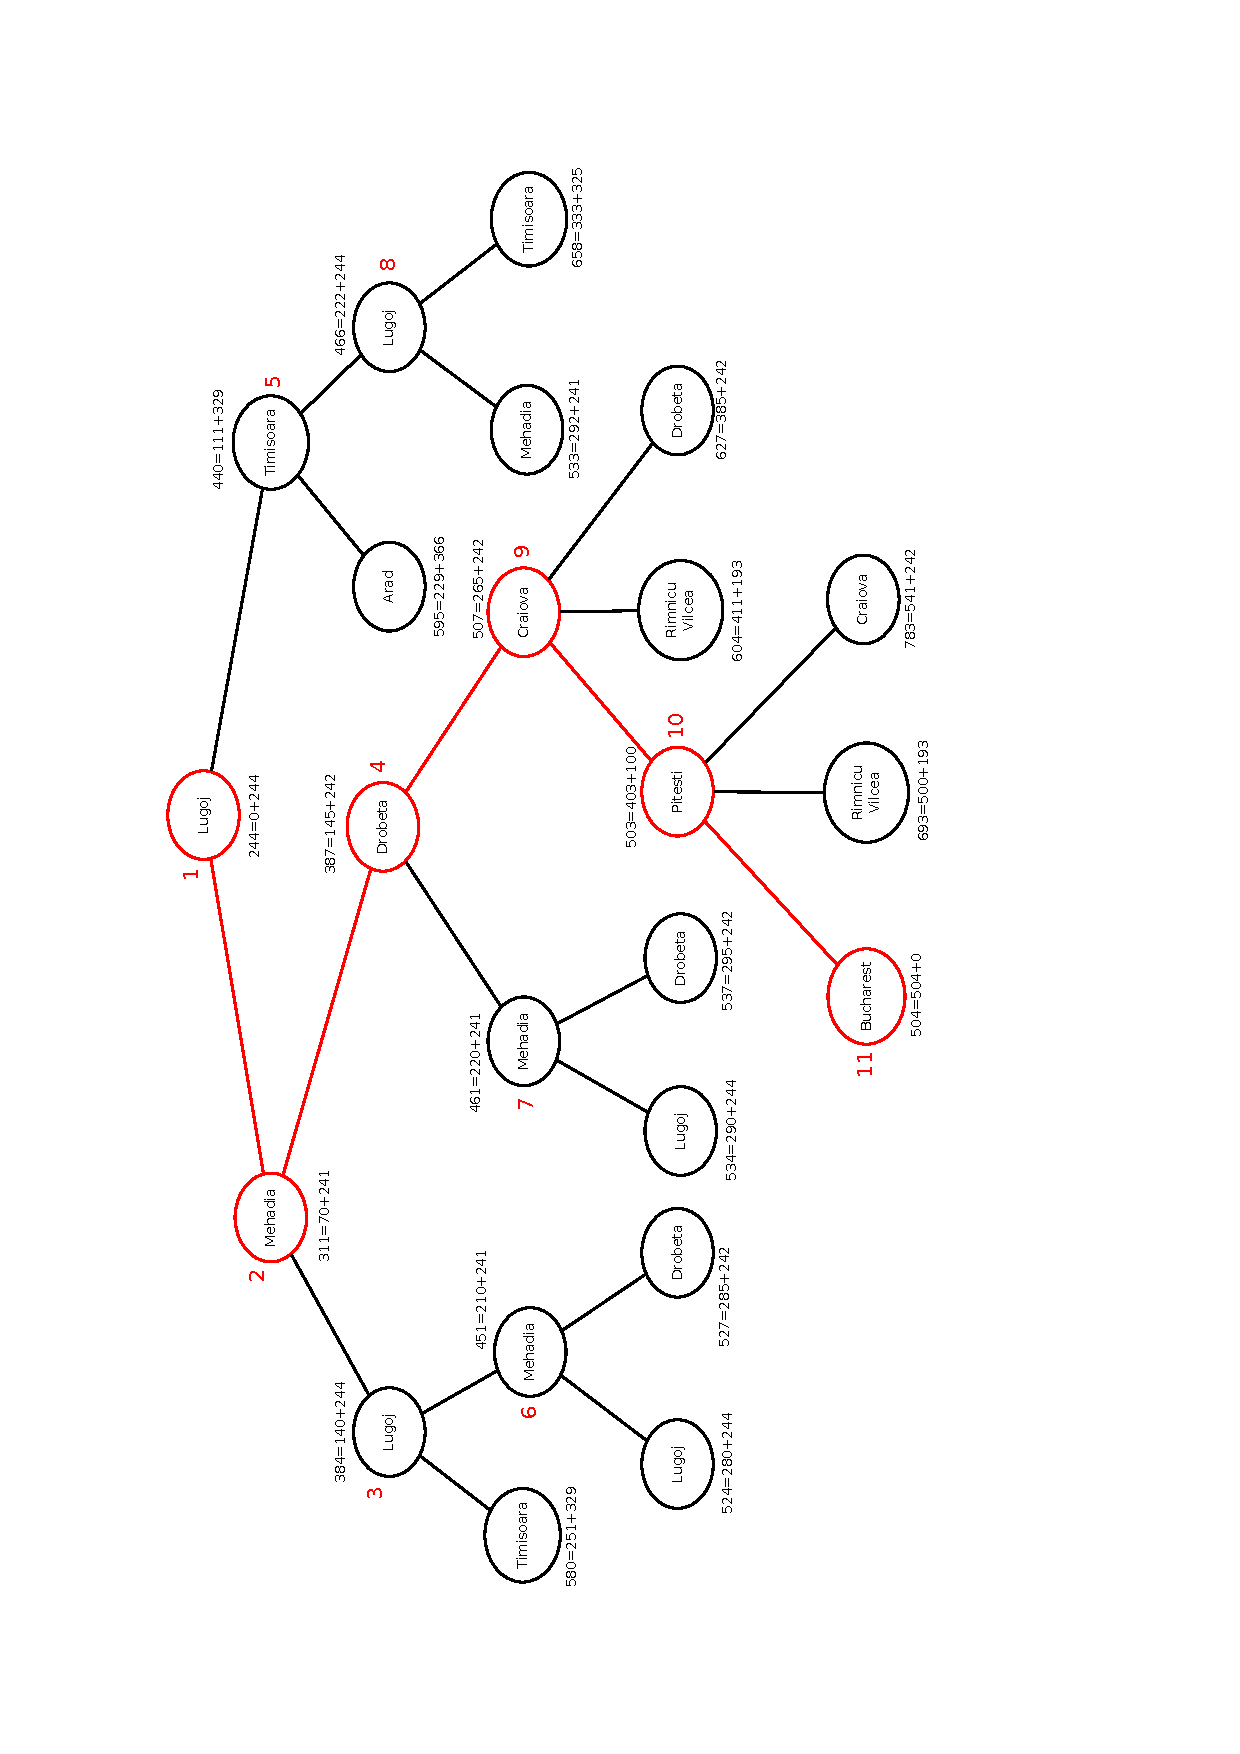
\includegraphics[width=0.55\textwidth, angle =-90, trim = 25mm 25mm 50mm 25mm,clip=true]{images/exercise3.pdf}}
\caption{Stages in an A* search from Lugoj to Bucharest. Nodes are labeled with $f = g+ h$ (black font), and with the selected order of expansion (red font). The sequence of states that are considered during each iteration consists of the current leaf nodes. The algorithm expands the leaf node with the lowest value of $f$, replacing it in the sequence with all its successors (to be considered for the following iteration). The optimal solution is depicted with red nodes and edges.}
\label{fig:exercise3}
% Place the label just after the caption to make the link work
\end{sidewaysfigure} % table makes a floating object with a title


\section*{Exercise 4}

\subsection*{Part A}

Since only one state ($k=1$) is stored in memory after each iteration, it is iteratively succeeded by its best neighboring state like in hill climbing. Hence, the local beam search algorithm with $k=1$ is a simple hill climbing algorithm.

\subsection*{Part B}

With temperature $T=0$, we can say that the probability $e^{\Delta E/T}=0$ when $\Delta E \le 0$, namely only better neighboring solutions are accepted. Therefore, simulated annealing with $T=0$ is a first choice hill climbing algorithm.

\subsection*{Part C}

If $N=1$, the population will consist of a single individual. Crossover will thus happen between (two copies of) that individual, resulting in the exact same solution. The random mutation mechanism will introduce a small number of point changes during each iteration, consequently turning genetic algorithm into a random walk.






